\documentclass{article}
\usepackage{graphicx}
\usepackage{amsmath}
\usepackage{cite}
\usepackage{color}
\usepackage{enumitem}
\usepackage{hyperref}
\usepackage{natbib}
\usepackage{tabularx}
\usepackage{natbib}
\usepackage{ragged2e}

\title{\textbf{"Principi di Reti Neurali"}}
\author{Alessandro Meloni GEPID}
\date{}
\begin{document}
\maketitle
\begin{abstract}
\begin{justify}
    Questo paper si soffermerà sull'analisi, la nascita, l'evoluzione delle reti neurali e i principi del loro funzionamento. Il punto focale sarà sicuramente quello di capire quanto un'intelligenza artificiale di questa portata, possa influire sul lavoro e la relativa organizzazione.In relazione a ciò, comprendere finquanto esse si possano spingere, quanta concorrenza potrebbero generare e i risvolti positivi/negativi sulla domanda di lavoro.
\end{justify}
\end{abstract}
\centering \tableofcontents
\centering \newpage
\section{Le Reti neurali}
\flushleft \subsection{Cosa sono?}
\begin{justify}
    Le reti neurali sono delle vere e proprie rappresentazioni informatiche, il quale funzionamento è paragonabile alla funzione e il comportamento che hanno i nostri neuroni biologici nel cervello.\\
    Molto probabilmente parlando di reti neurali, la maggior parte delle persone, non sa neanche che attualmente ne abbiamo tante in circolazione; e una tra le tante, che sicuramente ha acquisito una forte influenza, sia positiva che negativa, è ChatGpt.\\
    A parte questa piccola introduzione, noi chiamiamo le reti neurali in svariati modi, chi le chiama AI, chi le chiama con l'acronimo ANN (artificial neural network), oppure ancora SNN (simulated neural network).\citep{IBM2021} \\
    Indipendentemente dal nome che gli viene assegnato, le classifichiamo all'interno del mondo del Machine Learning (un linguaggio ad alta astrazione che ti da la possibilità, imparando da dei modelli attuali, di poter fare delle opportune previsioni future).\\
    A sua volta però risulta essere il perno di ulteriori algoritmi che vengono chiamati "deep learning": meccanismo algoritmico utilizzato dalle AI per modellare il funzionamento delle reti neurali, attraverso anche l'attribuzione di weights e biases; per esempio: riconoscere delle immagini, saper descrivere gli elementi chiave di un immagine, elementi di testo, suoni e via discorrendo.\citep{AWS2022}
\end{justify}


\flushleft\subsection{Evoluzione cronologica}
\flushleft 
\begin{justify}
    Dal punto di vista storico le reti neurali hanno una portata molto ampia, però, anche se le prime teorie di una "macchina che pensa" possano essere fatte risalire agli antichi greci, noi ci soffermeremo esclusivamente sui passaggi chiavi: così da avere una buona visione su questi aspetti. Suddivideremo questi punti in ordine cronologico:
\begin{itemize}
    \item \textbf{1943:}In quest'anno venne pubblicata una ricerca, che è poi quella fondamentale, dando vita al primo concetto di rete neurale. L'articolo con il nome: "A logical calculus of the ideas immanent in nervous activity", venne pubblicato da Warren McCulloch e Walter Pitts (neurofisiologo e matematico statunitense). Egli cercarono di comprendere come il cervello riesca a elaborare dei modelli complessi attraverso l'interconnessione neurale. Il risultato della ricerca che a noi interessa è che, il loro funzionamento, venne paragonato a una soglia binaria e all'algebra di Bool.\citep{mcculloch1943logical}
    \item \textbf{1958:}Con la ricerca: "The Perceptron: A Probabilistic Model for Information Storage and Organization in the Brain" istituita da Frank Rosenblatt (psicologo statunitense), riuscì a portare avanti la ricerca precedente, introducendo il meccanismo dei pesi all'interno dell'equazione\citep{rosenblatt1958perceptron}.
    Importante anche lo sviluppo del percettrone: \textit{"Il percettrone fu proposto da Frank Rosenblatt nel 1958 come un'entità con uno strato di ingresso ed uno di uscita ed una regola di apprendimento basata sulla minimizzazione dell'errore, la cosiddetta funzione di error back-propagation (retropropagazione dell'errore) che in base alla valutazione sull'uscita effettiva della rete rispetto ad un dato ingresso altera i pesi delle connessioni (sinapsi) come differenza tra l'uscita effettiva e quella desiderata".}\href{https://it.wikipedia.org/wiki/Percettrone}{Rimando alla definizione su wikipedia}
    \item \textbf{1974:}Il ricercatore che poi riuscì ad applicare nel concreto, e per la prima volta, il meccanismo di retropropagazione, fu Paul Werbos, attraverso la sua tesi di dottorato. La retropropagazione indica un algoritmo utilizzato per l'addestramento delle reti neurali artificiali, combinato con un metodo di ottimizzazione chiamato "discesa stocastica del gradiente (\textit{...ad ogni iterazione, sostituisce il valore esatto del gradiente della funzione costo con una stima ottenuta valutando il gradiente solo su un sottinsieme degli addendi}\citep{werbos1990backpropagation}
    \item \textbf{1989 ad oggi:} Infine ricordiamo Yann LeCun che in un articolo pubblicato nel 1989 circa, tentò di spiegare come il meccanismo di retropropagazione funzioni e come possa essere integrato nella struttura della rete neurale per addestrare gli algoritmi\citep{lecun1989backpropagation}. Al giorno d'oggi, tutto questo che abbiamo appena detto, fa parte della branca informatica del deep learning, che risulta essere, giorno dopo giorno, in continua evoluzione (ChatGpt, Grok, Assistenti vocali nei telefoni etc...).
\end{itemize}
\end{justify}
\centering \newpage
\section{Il funzionamento}

 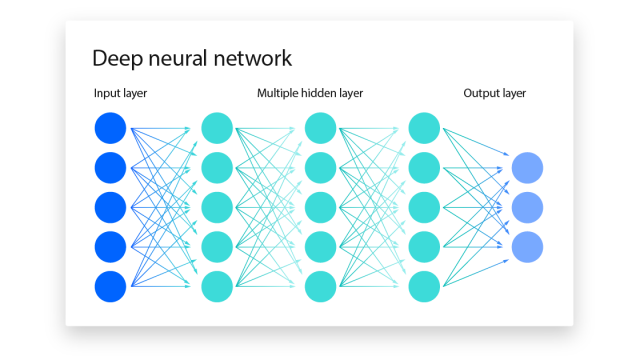
\includegraphics[width = 0.5\linewidth]{PROGETTO RETI NEURALI/ImmaginiProgetto/NeuNet.jpg}
    \label{F1:foto reti}

\flushleft \subsection{Come si comportano?}

\flushleft \subsection{A cosa servono?}
 
\flushleft \subsection{L'organizzazione e il mercato del lavoro}

\centering \newpage
\section{Considerazioni finali}
\bibliography{Database}
\bibliographystyle{alpha}
\end{document}
